\documentclass[DIV12,english,11pt,halfparskip]{scrartcl}
\usepackage[pdftex]{graphicx}
\usepackage[latin1]{inputenc}
\usepackage[headsepline]{scrpage2}
\usepackage{amsmath}
\usepackage{amssymb}
\usepackage{graphicx}
\usepackage{xcolor}
\usepackage{natbib}
%\usepackage{subfigure}
\usepackage[pdfpagemode=None,%
%linkbordercolor = 0 0 0,%
linkcolor = red,%
%anchorcolor = 0 0 0,%
citecolor = blue,%
%filecolor = 0 0 0,%
%5menucolor = 0 0 0,%
%pagecolor = 0 0 0,%
urlcolor = violet,%
colorlinks,%
plainpages=false, pdfpagelabels,%
%backref,%
pdftitle={JANE - System Architecture and Installation HowTo},%
pdfsubject={},%
pdfauthor={Katrin Tomanek},%
pdfkeywords={Jena Annotation Environment, JANE},%
pdfcreator={JULIE Lab, University of Jena},%
pdfproducer={pdfeTeX},%
]{hyperref}
\pagestyle{scrheadings}
\automark{section}

\title{JANE -- System Architecture and Installation}

\author{\normalsize Katrin Tomanek\\
  \normalsize  Jena University Language \& Information Engineering (JULIE) Lab\\
  \normalsize F\"urstengraben 30 \\
  \normalsize D-07743 Jena, Germany\\
  {\normalsize \tt tomanek@coling-uni-jena.de} } \date{}

\begin{document}
\maketitle
\newpage
\tableofcontents
\newpage
\section{Introduction}

This is an installation howto of JANE, the Jena Annotation
Environment. Please follow the instructions carefully. The
installation assumes that you have a basic understanding of Linux.

\textbf{Important note}: Please run all components of JANE on Linux.
JANE has only been tested and used before on a Linux environment. JANE
is implemented in Java and could thus also be run on a Windows
machine. However, in this case the configuration settings (especially
paths) will have to be changed accordingly -- please note that we
won't be able to help you running JANE on Windows.

JANE requires Sun's Java 1.5. It will not run with older versions of
Java and has not been tested with Java 1.6.

Before installing JANE, have a look at JANE's system architecture in
section \ref{sec:architecture}. There, the important concepts and
components of JANE will be explained in short. JANE can be run on a
distributed environment, allowing the different components to be run
on different machines. This section will show as an example how JANE
is used in the JULIE Lab.



\section{System Architecture}
\label{sec:architecture}



\begin{figure}[h]
  \centering
  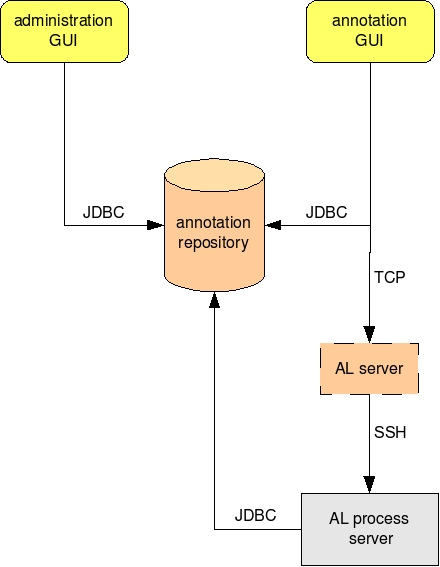
\includegraphics[scale=0.4]{figs/architecture.jpg}
  \caption{JANE system architecture}
  \label{fig:architecture}
\end{figure}


Figure \ref{fig:architecture} shows the general system architecture of
JANE. From a technical point of view, JANE consists of the following components:

\begin{itemize}
\item annotation GUI -- a tools for the annotators to do the
  annotations (sometimes also called AnnoClient)
\item administration GUI -- a tool for annotation administrators to
  create projects, monitor the annotation process, deploy annotations
  etc. (sometimes also called AnnoMaster)
\item annotation repository -- a MYSQL database where all annotations
  and related data is stored
\item AL server -- a small server program that listens on a given TCP
  port for incoming AL selection requests. When it gets such a request
  it prepares the AL selection and hands the actual AL selection task
  to the AL process server (via an SSH call)
\item AL process server -- the machine where the actual AL selection
  task is being run (typically a high-performant machine with lots of
  memory).
\end{itemize}

When not talking about JANE in a technical manner, we typically
simplify and refer to the AL server and the AL process server as one
component (also called '\emph{AL server}' then).

All components communicate via network, three different protocolls are
used (JDBC for connections to the annotation repository, a simple TCP
based protocoll for requests to the AL server, and an SSH call to
start the actual AL selection process). Thus, JANE can easily be run
in a distributed environment enabling e.g. annotators to work remote
(from at home or another lab).

Figure \ref{fig:installation_julielab} shows the installation of JANE
at the JULIE Lab: in our case, both the annotation repository, the AL
server, and the AL process server are on the same (physical) machine
(called the ``annotation machine'' here). The administration GUI and
the annotation GUI are installed so that they can be opened from all
desktop PCs in our lab.


\begin{figure}[bt]
  \centering
  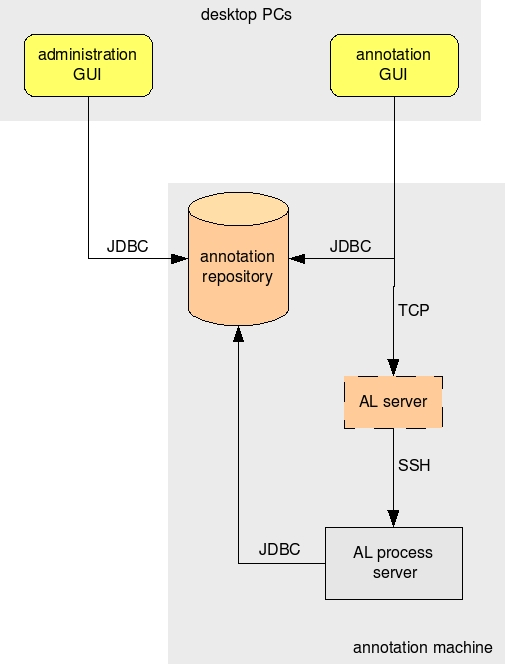
\includegraphics[scale=0.4]{figs/architecture_julielab.jpg}
  \caption{JANE: installation at JULIE Lab}
  \label{fig:installation_julielab}
\end{figure}


Thus, on which machines you install which components depends highly on
your needs. The most simple installation is one where all components
are run at the same machine.


% introduce concepts and terminology
% installation in julie lab


\section{Installing JANE}
\label{sec:installation}

Installing JANE consists of the following four steps: unpacking the
downloaded package (step 1), installing the annotation repository
(step 2), configuring the components of JANE (step 3), starting the
active learning server (step 4).


% SSH key


\subsection{Unpacking JANE}

To install JANE, unpack the \url{tgz} file you have
downloaded.  A new directory (\url{JANE-1.0)} is created. The
directory will have the following file and directory structure:

\begin{verbatim}
 bin            -> contains scripts to run the single components of JANE
 demo           -> demo data for a default project
 doc            -> documentation (user howtos, installation guide)
 install        -> installation stuff 
 lib            -> java libraries used (JANE, and also external ones)
 lib/MMAX2_1.1  -> libraries for MMAX2
 resources      -> external resources (such as POS dictionary)
 settings       -> configuration files for the single components of JANE
\end{verbatim}


\subsection{Annotation Repository}
\label{ss:install_annorep}

\textsc{JANE} requires a MYSQL database (tested only with MYSQL
version 5.0) for the annotation repository.  Ask your system
administrator in case MYSQL is not installed.

Then, you need to create an empty annotation repository. Therefore,
just import the MYSQL dump of the initial annotation repository, which
you will find in the directory \url{install} directory:

\begin{enumerate}
 \item create a database 'myJaneDB' on your MYSQL server
\begin{verbatim}
   mysql> create database myJaneDB;
   Query OK, 1 row affected (0.00 sec)
\end{verbatim}

 \item add a user to your MYSQL database that has all privileges on
   this database (replace '\emph{JaneDBUser}' and
   '\emph{JaneDBUserPassword}' by some other name and password).
\begin{verbatim}
   mysql> grant all on myJaneDB.* to 'JaneDBUser'@'%'
          identified by 'JaneDBUserPassword';
   Query OK, 0 rows affected (0.00 sec)

   mysql> flush privileges;
   Query OK, 0 rows affected (0.00 sec)
\end{verbatim}

 \item no go back to the command line and import the MYSQL dump from
   the install directory
\begin{verbatim}
    tomanek@localhost:/home/tomanek/JANE-1.0/install$ mysql 
           -u JaneDBUser -p myJaneDB < myJaneDB.sql
\end{verbatim}
\end{enumerate}


The initial annotation repository is empty except that it contains the
administrator user '\emph{admin}' for JANE with the passwort
'\emph{admin}'\footnote{In case you want to change the password of the
  administrator, you will have to do this in the MYSQL database
  directly by editing table 'user' with any MYSQL client.}. You can
now go to the administration GUI and add further users and annotation
projects.

  Furthermore, a test user (password '\emph{test}') and a test
  annotation project have been added to the initial repository. After
  installation is complete, start the annotation GUI, login as user
  '\emph{test}' and check whether you can successfully open and
  annotate the test project.



\subsection{Configuration}

After unpacking JANE (step 1) you need to configure its single
components. You will find the following configuration files in the
subdirectory \url{settings}\footnote{Note: make sure, that these files
  exist, otherwise JANE will not work properly.}:
\begin{itemize}
\item \url{database.properties} -- defines how to access the
  annotation repository
\item \url{annoclient.properties} -- settings for the annotation GUI
\item \url{annomaster.properties} -- settings for the administration
  GUI
\item \url{annomaster.tooltips} -- tooltips to be shown in
  administration GUI; nothing has to be changed here!
\item \url{activelearning.properties} -- settings for active learning selection
\item \url{logging.properties} -- do not change anything here!
\end{itemize}

These files contain pairs of configuration keys with their respective
values. The order of the keys in the file doesn't matter. This section
contains a description of the respective keys and their meaning. Use
the configuration scripts from the subdirectory \url{install} to
modify these files. After an initial configuration of these files,
some values can also be modified manually in a text editor.


\subsubsection{Database Settings}

Run the script \url{configureDBSettings.sh}. You will be asked for the
following configuration parameters:

\begin{description}
\item [DB location] enter the path to your annotation repository as
  URL. This has the following format 
\begin{verbatim}
  jdbc:mysql://<server-ip>/<db-name>
\end{verbatim}
  where '\emph{server-ip}' is the IP of the server where you have
  installed the MYSQL server and '\emph{db-name}' is the name of your
  MYSQL database used as annotation repository (if you used the MYSQL
  dump to create your initial annotation repository, this will be
  '\emph{myJaneDB}').
\item[DB user] enter the DB user (step 2: '\emph{JaneDBUser}') you
  have created when installing the initial annotation repository.
\item[DB password] enter the password for the DB user (step 2:
  '\emph{JaneDBUserPassword}').
\end{description}

Now, the parameters you specified will be checked, i.e., the
configuration scripts tries to open a connection to your annotation
repository. If this succeeds, the database settings where successfully
configured. Otherwise you will have to re-run the script.

Note: these settings are stored in \url{database.properties}; the
password is encrypted.


\subsubsection{Annotation GUI Settings}
Run the script \url{configureAnnotationGUI.sh}. You will be asked for
the following configuration parameters:

\begin{description}
\item [Base directory of JANE] enter the complete path to your JANE
  installation. Finish it with a slash (``/'').

  Example: when I unpack JANE in my home directory (\url{/home/tomanek})
  I would have to write: \url{/home/tomanek/JANE-1.0/}

\item[Directory for temporary files] enter the complete path to a
  directory (you need write access) where JANE can store
  temporary files. Just press enter to accept the default (\url{/tmp}).

\item[Directory with MMAX libraries] MMAX2 is the annotation editor
  used by JANE. You can use the MMAX2 libraries provided with JANE.
  These are contained in the subdirectory \url{libs/MMAX2_1.1}.  You
  have to enter the full path to the MMAX2 libraries.

  Example: I might enter
  \url{/home/tomanek/JANE-1.0/lib/MMAX2_1.1}
\end{description}

You can further manually change the following parameters by editing the file
\url{annoclient.properties} (do not delete any keys!):

\begin{description}
 \item[mmax.mem] the memory you want MMAX2 allow to use (default is 256m)
 \item[ac.refresh\_interval] time interval to refresh AL log output in
   seconds (default is 5 seconds)
 \item[autosave.interval] time interval for saving modifications made
   during annotation to the annotation repository (default is 60 seconds)
\end{description}


\subsubsection{Administration GUI Settings}
Run the script \url{configureAdministrationGUI.sh}. You will be asked for
the following configuration parameters:

\begin{description}

\item [Base directory of JANE] enter the complete path to your JANE
  installation (same as for annotation GUI). Finish it with a slash
  (``/'').

  Example: if I unpack JANE in my home directory (\url{/home/tomanek})
  I would have to write: \url{/home/tomanek/JANE-1.0/}

\item[Directory for temporary files] enter the complete path to a
  directory (you need write access) where JANE can store
  temporary files. Just press enter to accept the default (\url{/tmp}).

\item[Directory with POS dictionary] enter the relative path to the
  base directory of JANE. Just press enter to accept the default value
  (\url{resources/POS/}).
\end{description}


\subsubsection{Active Learning Settings}
There is no configuration script for the active learning settings,
yet. So you have to manually edit the file
\url{activelearning.properties}. The following parameters have to be
specified:

\begin{description}
\item[alserver.tmpdir] full path to a directory where temporary data
  can be stored (make sure this directory exists and the user can read
  and write to it)
\item[alserver.host] the hostname (better: IP address) of the computer
  where the AL server is running
\item[alserver.port] the port of the AL server (make sure it doesn't
  collide with other applications, thus: don't use well-known ports
  and ask you administration to make sure the respective port is
  unused and not blocked by a firewall)
\item[al.process-server] the AL server can run the actual AL selection
  process on another (high-performant) machine, the AL process server.
  Add the hostname (better: IP address) of the machine where the AL
  selection process should be run
\item[al.path] full path to your installation of JANE on the AL
  process server
\item[al.mem] specify the amount of memory you want the AL selection
  process to use (make sure, that the AL process server where you run the AL
  selection process, has the respective mount of memory, otherwise AL
  selection will not work!)
\end{description}

Note: in most cases, the AL server and the AL process server can be
run on the same machine. However, in case the machine where the AL
selection process should be run is not accessable from 'outside' but
you want remote users to be able to run AL, you might set up the AL
server on a machine which can be connected from outside. See the
architecture overview for a better understanding.


\subsection{Starting the Active Learning Server}
The AL server is a small program that listens on a specified TCP port
for AL selection requests. It then runs the AL selection process on
the AL process server by means of an \url{SSH} call. 

Note: for running the AL selection process the same user as for the AL
server must exist on the AL process server!

Further, you should generate an ssh-key (without a passphrase) for the
user on the AL server which has started the AL server to avoid the AL
server waiting for you to enter a password when it hands the AL
selection process to the AL process server. Having created the ssh-key,
you have to add the ssh-key (public key) to the list of authorized
keys on the AL process server of the respective user (must be the same
user as for the AL server).

Once, this is done, you can start the AL server by calling
\url{runALServer.sh} from the directory \url{bin}. We typically run
the AL server with the \url{screen} command (using \url{screen}, you
can detach and reattach sessions\footnote{Also see the \url{screen}
  howto of your Linux distribution.}):

\begin{verbatim}
screen -S "JANE AL server" ./runALServer.sh
\end{verbatim}

Make sure your AL server is running\footnote{Note: \url{screen}
  sessions sometimes 'die' after some days; in such a case, just
  restart the AL server.}. Otherwise, annotators will get an error when
sending an AL request. In case there are any errors with the AL
selection although the AL server is running, it is a good starting
point to check the output of the AL server (therefore, you might want
to dettach your \url{screen} session).


\section{Copyright and License}

This software is Copyright (C) 2007 Jena University Language \&
Information Engineering Lab (Friedrich-Schiller University Jena,
Germany). It can be used free of charge for academic non-commercial,
non-profit research purposes only. If you want to use JANE other than
in the demo version you have to fill out and send us the license
agreement
(\url{https://watchtower.coling.uni-jena.de/~tomanek/coling/JANE/JULIE_JANE_LICENSE.pdf}).

JANE is provided on an ``as is'' basis, without any warranties or
conditions of any kind. Each recipient is solely responsible for
determining the appropriateness of using JANE.

Further, please note that JANE-1.0 is still a beta version!

\end{document}
